\chapter[Resultados Parciais]{Resultados Parciais}

\section{Protótipo inicial}

A fim de atestar a viabilidade do porte do jogo \textit{Traveling Will}, desenvolvido inicialmente para PC, para a plataforma \textit{Nintendo Game Boy Advance}, foi feita uma versão funcional do menu original do jogo, tendo essa versão sido testada em um GBA real. Para isso, a principal ferramenta utilizada foi a libtonc \cite{libtonc}, que nessa versão inicial fez o papel de engine do jogo.

Abaixo é possível comparar o menu principal do jogo original com o protótipo implementado sendo executado em um emulador de \textit{Game Boy Advance}:

\begin{figure}[H]
 \centering \includegraphics[keepaspectratio=true,scale=0.6]{figuras/tw-original-1.eps}
   \caption{Jogo original \textit{Traveling Will} sendo executado em um PC. Fonte: \textit{Autores}.}
   \label{tw-original-1}
\end{figure}

\begin{figure}[H]
 \centering 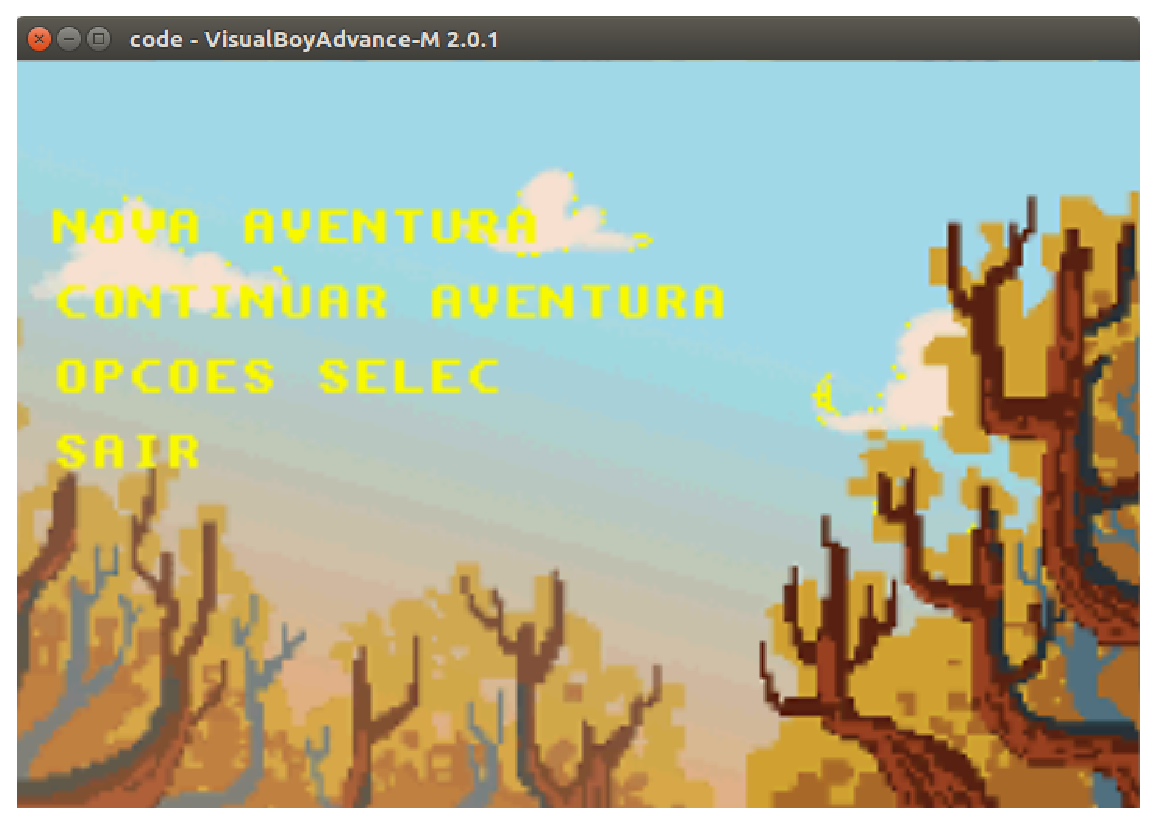
\includegraphics[keepaspectratio=true,scale=0.6]{figuras/tw-gba-1.eps}
   \caption{Protótipo implementado sendo executado em um emulador de GBA. Fonte: \textit{Autores}.}
   \label{tw-gba-1}
\end{figure}

\section{Desenvolvimento da \textit{engine}}

Após a finalização do protótipo inicial, foi iniciado o desenvolvimento da engine que irá substituir a libtonc na versão final do jogo. Ela irá padronizar a utilização dos recursos providos pelo GBA e irá conter um módulo de vídeo, áudio, \textit{input}, física, dentre outros.

Até o momento, o módulo de \textit{input} e parte do módulo de vídeo foram implementados.

\subsection{Módulo de \textit{input}}

Os estados dos botões do GBA ficam salvos em um registrador. Cada um desses estados é representado por um \textit{bit} no valor guardado por esse registrador. Sempre que um botão é apertado, o GBA automaticamente troca o valor guardado nesse registrador de tal forma que o \textit{bit} que representa o botão em questão passe a possuir valor 0. De forma similar, quando o botão é solto, o valor contido no \textit{bit} em questão é modificado para 1, seu valor padrão. Sendo assim, a checagem dos estados pode ser realizada facilmente utilizando \textit{bitmasks}. Por exemplo, caso se deseje checar um botão representado pelo \textit{bit} 2 (com a contagem começando em 0), basta pegar o resultado do \textit{AND} binário entre o valor guardado no registrador e a potência de 2 que possui como expotente o \textit{bit} em questão (4, nesse exemplo). Abaixo é possível vizualizar no código do módulo de input a definição das constantes que representam os botões, assim como a função utilizada para checar o estado de cada um deles:

\begin{minted}[frame=lines, linenos]
{c++}
#ifndef INPUT_H
#define INPUT_H

#include <stdbool.h>
#include "base_types.h"

#define BUTTON_A 1
#define BUTTON_B 2
#define BUTTON_SELECT 4
#define BUTTON_START 8
#define BUTTON_RIGHT 16
#define BUTTON_LEFT 32
#define BUTTON_UP 64
#define BUTTON_DOWN 128
#define BUTTON_R 256
#define BUTTON_L 512

#define N_BUTTON 10

int pressed_state[N_BUTTON];

void check_buttons_states();
bool pressed(int button);

#endif
\end{minted}
\makebox[\width]{Cabeçalho do módulo de input. Fonte: \textit{Autores}.}

\begin{minted}[frame=lines, linenos]
{c++}
#include "input.h"

volatile unsigned int *buttons_mem = (volatile unsigned int *)0x04000130;

void check_buttons_states() {
    for(int i = 0; i < N_BUTTON; i++) {
        pressed_state[i] = !((*buttons_mem) & (1 << i));
    }   
}

bool pressed(int button) {
    return pressed_state[button];
}
\end{minted}
\makebox[\width]{Código fonte do módulo de input. Fonte: \textit{Autores}.}

\subsection{Módulo de vídeo}

O módulo de vídeo deve possuir funções para controle do modo de vídeo, dos \textit{backgrounds} e da renderização das \textit{sprites}. Atualmente o módulo de vídeo desenvolvido trata apenas, de forma limitada, do modo de vídeo e do \textit{background}. Ele permite a renderização de um determinado \textit{background} desde que sejam passados a paleta de cores utilizada, um vetor com os \textit{tiles} utilizados no \textit{background} e um vetor representando o mapa de \textit{tiles} a ser utilizado para renderizar o \textit{background}. O módulo copia cada uma das informações passadas para as regiões de memória apropriadas. Atualmente, o módulo sempre utiliza o \textit{background} 2 e parte do princípio de que o modo utilizado não é baseado em \textit{bitmap}, não permitindo, portanto, o uso de múltiplos \textit{backgrounds}. Além disso, o módulo ainda não permite definir a posição exata de memória aonde o vetor de \textit{tiles} e o \textit{tilemap} deverão ser escritos, o que inviabiliza o uso de diferentes \textit{tilemaps}. Abaixo é possível visualizar a versão atual do código fonte do módulo de vídeo:

\begin{minted}[frame=lines, linenos]
{c++}
#include "video.h"

#include <string.h>

void reset_dispcnt() {
  REG_DISPCNT = 0;
}

void set_video_mode(int video_mode) {
  REG_DISPCNT |= video_mode;
}

void set_background_number(int background) {
  switch (background) {
    case 0:
      REG_DISPCNT |= 0x0100;
    case 1:
      REG_DISPCNT |= 0x0200;
    case 2:
      REG_DISPCNT |= 0x0400;
    case 3:
      REG_DISPCNT |= 0x0800;
  }
}

void set_background(const void *pal, int pal_len, const void *tiles, int tiles_len, const void *map, int map_len) {
  // Load palette
  memcpy(pal_bg_mem, pal, pal_len);
  // Load tiles into CBB 0
  memcpy(&tile_mem[0][0], tiles, tiles_len);
  // Load map into SBB 31
  memcpy(&se_mem[31][0], map, map_len);

  REG_BG2CNT = BG_CBB(0) | BG_SBB(31) | BG_8BPP | BG_REG_64x32;
}
\end{minted}
\makebox[\width]{Código fonte do módulo de vídeo. Fonte: \textit{Autores}.}
